\section{Approach}
	In this section we will present our aproach to tackle the speaker recognition problem.
	There're two steps in a complete speaker recognition system: enrollment and recognition.
\subsection{Erollment}
	\label{sec:approach_enrollment}
	An utterance of a user is collected during enrollment procedure.
	Further processing of the utterance follows following steps:
	\begin{enumerate}
		\item \textbf{Voice Activity Detection (VAD)} \\
			An observation found is that, the corpus provided by teacher is
			nearly noise-free. Therefore we use a simple energy-based approach
			to remove the silence part. We divide the utterance into 20ms frames,
			and remove the frames that the average energy is below 0.01 times
			the average energy of the whole utterance.

		\item \textbf{Extract MFCC and LPC Features} \\ We extract
			Mel-frequency cepstral coefficients(MFCC) and Linear Predictive
			Coding (LPC) features using following parameter found to be
			optimal:

			\begin{itemize}
				\item Common parameters:
					\begin{itemize}
						\item Frame size: 32ms
						\item Frame shift: 16ms
						\item Preemphasis coefficient: 0.95
					\end{itemize}
				\item MFCC parameters:
					\begin{itemize}
						\item number of cepstral coefficient: 19
						\item number of filter banks: 55
						\item maximal frequency of the filter bank: 6000
					\end{itemize}
				\item LPC Parameters:
					\begin{itemize}
						\item number of coefficient: 15
					\end{itemize}
			\end{itemize}

			and then concatenate the two feature vectors of the same frame forming
			a larger feature vector of 19 + 15 = 34 dimension.

		\item \textbf{Gaussian Mixture Model}
			We use Gaussian Mixture Model modeling a speaker. Some improvements made:
			\begin{itemize}
				\item Performance: \\
					We investigate the effect of initialization of GMM during
					training. We implemented GMM with
					K-meansII\cite{bahmani2012scalable}, which is an improved
					version of K-means++\cite{arthur2007k} to initialize the
					mean vector of GMM. Results shows improvements compared
					to GMM provided by \textbf{scikit-learn\cite{scikit-learn}}.
				\item Efficiency: \\
					\begin{itemize}
						\item We provide a parallel version of GMM, especially
							optimized to train large Universal Background Model(UBM).
						\item We further improve efficiency by utilizing
							SSE instruction in computing exponential function
							using polynomial approximation. This can speed up
							the training procedure by a factor of two.
					\end{itemize}

		\item \textbf{Universal Background Model}
			As we are providing continuous speech close-set diarization function in
			GUI, we adopt Universal Background Model(UBM) as imposter model,
			and use likelihood ratio test to make reject
			decisions.\cite{reynolds2000speaker}

			When using conversation mode in GUI (will be present later),
			GMM model of each user is adapted from a pre-trained UBM
			using method described in \cite{reynolds2000speaker}.

		\item \textbf{Continuous restricted Boltzmann Machine(CRBM)}

			Restricted Boltzmann Machine(RBM) is generative stochastic
			two-layer neural network that can learn a probability distribution
			over its set of binary inputs\cite{rbm_wiki}.  Continuous
			restricted Boltzmann Machine(CRBM)\cite{chen2003continuous} extends
			its ability to real-valued inputs.  RBM has a ability to, given an
			input(visible layer), reconstruct a visible layer that is similar
			to the input.  \figref{crbm} illustrate original MFCC data and the
			sampled output of
			reconstructed data from CRBM.
			\begin{figure}[!ht]
				\label{fig:crbm}
				\begin{minipage}{0.48\linewidth}
					\centering
					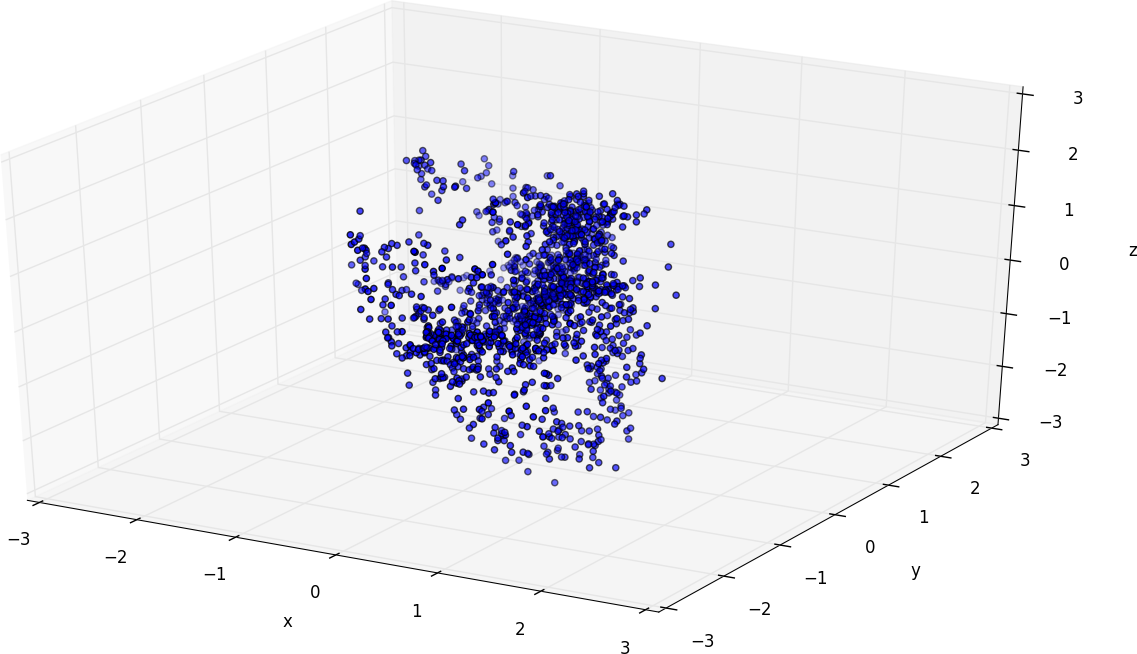
\includegraphics[width=\linewidth]{res/all.trimed.png}
					\caption{The first three dimension of a woman's MFCC feature}
				\end{minipage}
				\hfill
				\begin{minipage}{0.48\linewidth}
					\centering
					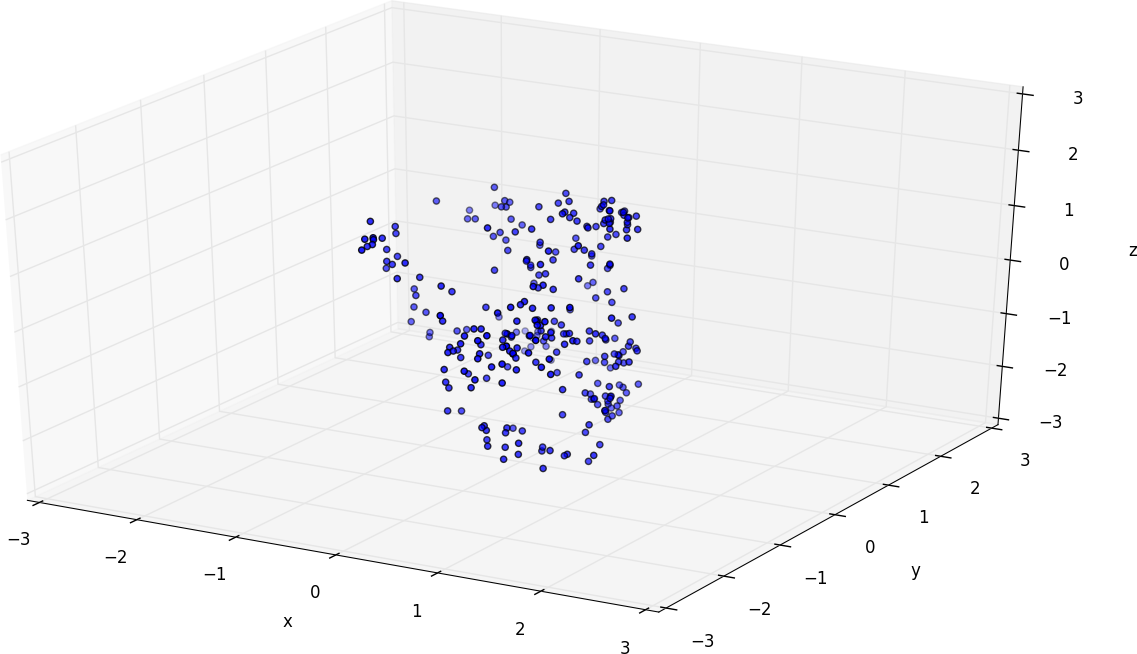
\includegraphics[width=\linewidth]{res/50.trimed.png}
					\caption{The first three dimension of the same woman's MFCC feature
					recontructed by a CRBM with 50-neuron hidden layer. We can
					see that, the density of these two distributions are alike}
				\end{minipage}
			\end{figure}


		\item \textbf{JFA}:
			% TODO: wyx shorter version

          \textbf{Factor Analysis} is a typical method which behave
          very well in classification problems, due to its ability to
          account for different types of variability in training data.
          Within all the factor analysis methods,
          Joint Factor Analysis (JFA)\cite{jfa2,jfa-se} was proved to outperform other method
          in the task of Speaker Recognition.

          JFA models the user by ``supervector'' , i.e. a $C\times F $ dimension vector, where $C$ is
          the number of components in the Universal Background Model, trained by GMM on all the training data,
          and $ F$ is the dimension of the acoustic feature vector. The supervector of an utterance is obtained by concatenate
          all the $C $ means vectors in the trained GMM model. The basic assumption of JFA on describing a supervector is:

          \[ \vec{M} = \vec{ m } + vy + dz + ux, \]

          where $m$ is a supervector usually selected to be the one trained from UBM, $v$ is a $ CF \times R_s$ dimension matrix,
          $ u$ is a $ CF \times R_c$ dimension matrix, and $d$ is a diagonal matrix.
          This four variables are considered independent of all kinds of variabilities and remain constant after training, and
          $x, y, z $ are matrixes computed for each utterance sample.
          In this formulation, $ m + vy + dz$ is commonly believed to account for the ``Inter-Speaker Variability'', and $ux $ accounts
          for the ``Inter-Channel Variability''.
          The parameter $ R_s $ and $ R_c$, also referred to as ``Speaker Rank'' and ``Channel Rank'', are two emprical constant selected as first.
          The training of JFA is to calculate the best $ u, v, d$ to fit all the training data.

          After our investigation, we found that the original algorithm \cite{jfa-se} for training JFA model is of
          too much complication and hard to implement.
          Therefore, we use the simpler algorithm presented in \cite{jfa-study}
          to train the JFA model. However, from the result, JFA does not seem to outperform our enhanced MFCC and GMM algorithms
          (but do outperform our old algorithms). It is suspected that the training of a JFA model needs more data than
          we have provided, since JFA needs data from various source to account for different types of variabilities.
          Therefore, we might need to add extra data on the training of JFA, but keep the same data scale in the stage of enrollment,
          to get a better result.

          It is also worth mentioning that the training of JFA will take much longer time than our old method,
          since the estimation process of $ u, v, d$ does not converge quickly. As a result, it might not be practical to add
          JFA approach to our GUI system. But we will still test further on the performance of it, compared to other methods.
	\end{enumerate}

\subsection{Recognition}
	Recognition procedure follows steps below:
	\begin{enumerate}
		\item Record a short utterance of the speaker (typically less than 5 seconds)
		\item Preprocess the utterance using first two steps described in
			\secref{approach_enrollment}, e.g, VAD, MFCC and LPC feature extraction.
		\item Compute the `score' of each person enrolled, and adopt person
			corresponding the model which gives highest score to be the
			recognition result.

			A typical form of score is log-likelihood (or energy in RBM case).
	\end{enumerate}
